% Options for packages loaded elsewhere
% Options for packages loaded elsewhere
\PassOptionsToPackage{unicode}{hyperref}
\PassOptionsToPackage{hyphens}{url}
%
\documentclass[
  ignorenonframetext,
  compress, aspectratio=149]{beamer}
\newif\ifbibliography
\usepackage{pgfpages}
\setbeamertemplate{caption}[numbered]
\setbeamertemplate{caption label separator}{: }
\setbeamercolor{caption name}{fg=normal text.fg}
\beamertemplatenavigationsymbolshorizontal
% remove section numbering
\setbeamertemplate{part page}{
  \centering
  \begin{beamercolorbox}[sep=16pt,center]{part title}
    \usebeamerfont{part title}\insertpart\par
  \end{beamercolorbox}
}
\setbeamertemplate{section page}{
  \centering
  \begin{beamercolorbox}[sep=12pt,center]{section title}
    \usebeamerfont{section title}\insertsection\par
  \end{beamercolorbox}
}
\setbeamertemplate{subsection page}{
  \centering
  \begin{beamercolorbox}[sep=8pt,center]{subsection title}
    \usebeamerfont{subsection title}\insertsubsection\par
  \end{beamercolorbox}
}
% Prevent slide breaks in the middle of a paragraph
\widowpenalties 1 10000
\raggedbottom
\AtBeginPart{
  \frame{\partpage}
}
\AtBeginSection{
  \ifbibliography
  \else
    \frame{\sectionpage}
  \fi
}
\AtBeginSubsection{
  \frame{\subsectionpage}
}
\usepackage{iftex}
\ifPDFTeX
  \usepackage[T1]{fontenc}
  \usepackage[utf8]{inputenc}
  \usepackage{textcomp} % provide euro and other symbols
\else % if luatex or xetex
  \usepackage{unicode-math} % this also loads fontspec
  \defaultfontfeatures{Scale=MatchLowercase}
  \defaultfontfeatures[\rmfamily]{Ligatures=TeX,Scale=1}
\fi
\usepackage{lmodern}

\usetheme[]{Montpellier}
\usecolortheme[]{dove}
\useinnertheme[]{rounded}
\useoutertheme[]{miniframes}
\ifPDFTeX\else
  % xetex/luatex font selection
\fi
% Use upquote if available, for straight quotes in verbatim environments
\IfFileExists{upquote.sty}{\usepackage{upquote}}{}
\IfFileExists{microtype.sty}{% use microtype if available
  \usepackage[]{microtype}
  \UseMicrotypeSet[protrusion]{basicmath} % disable protrusion for tt fonts
}{}
\makeatletter
\@ifundefined{KOMAClassName}{% if non-KOMA class
  \IfFileExists{parskip.sty}{%
    \usepackage{parskip}
  }{% else
    \setlength{\parindent}{0pt}
    \setlength{\parskip}{6pt plus 2pt minus 1pt}}
}{% if KOMA class
  \KOMAoptions{parskip=half}}
\makeatother

\usepackage{color}
\usepackage{fancyvrb}
\newcommand{\VerbBar}{|}
\newcommand{\VERB}{\Verb[commandchars=\\\{\}]}
\DefineVerbatimEnvironment{Highlighting}{Verbatim}{commandchars=\\\{\}}
% Add ',fontsize=\small' for more characters per line
\newenvironment{Shaded}{}{}
\newcommand{\AlertTok}[1]{\textcolor[rgb]{0.75,0.01,0.01}{\textbf{\colorbox[rgb]{0.97,0.90,0.90}{#1}}}}
\newcommand{\AnnotationTok}[1]{\textcolor[rgb]{0.79,0.38,0.79}{#1}}
\newcommand{\AttributeTok}[1]{\textcolor[rgb]{0.00,0.34,0.68}{#1}}
\newcommand{\BaseNTok}[1]{\textcolor[rgb]{0.69,0.50,0.00}{#1}}
\newcommand{\BuiltInTok}[1]{\textcolor[rgb]{0.39,0.29,0.61}{\textbf{#1}}}
\newcommand{\CharTok}[1]{\textcolor[rgb]{0.57,0.30,0.62}{#1}}
\newcommand{\CommentTok}[1]{\textcolor[rgb]{0.54,0.53,0.53}{#1}}
\newcommand{\CommentVarTok}[1]{\textcolor[rgb]{0.00,0.58,1.00}{#1}}
\newcommand{\ConstantTok}[1]{\textcolor[rgb]{0.67,0.33,0.00}{#1}}
\newcommand{\ControlFlowTok}[1]{\textcolor[rgb]{0.12,0.11,0.11}{\textbf{#1}}}
\newcommand{\DataTypeTok}[1]{\textcolor[rgb]{0.00,0.34,0.68}{#1}}
\newcommand{\DecValTok}[1]{\textcolor[rgb]{0.69,0.50,0.00}{#1}}
\newcommand{\DocumentationTok}[1]{\textcolor[rgb]{0.38,0.47,0.50}{#1}}
\newcommand{\ErrorTok}[1]{\textcolor[rgb]{0.75,0.01,0.01}{\underline{#1}}}
\newcommand{\ExtensionTok}[1]{\textcolor[rgb]{0.00,0.58,1.00}{\textbf{#1}}}
\newcommand{\FloatTok}[1]{\textcolor[rgb]{0.69,0.50,0.00}{#1}}
\newcommand{\FunctionTok}[1]{\textcolor[rgb]{0.39,0.29,0.61}{#1}}
\newcommand{\ImportTok}[1]{\textcolor[rgb]{1.00,0.33,0.00}{#1}}
\newcommand{\InformationTok}[1]{\textcolor[rgb]{0.69,0.50,0.00}{#1}}
\newcommand{\KeywordTok}[1]{\textcolor[rgb]{0.12,0.11,0.11}{\textbf{#1}}}
\newcommand{\NormalTok}[1]{\textcolor[rgb]{0.12,0.11,0.11}{#1}}
\newcommand{\OperatorTok}[1]{\textcolor[rgb]{0.79,0.38,0.79}{#1}}
\newcommand{\OtherTok}[1]{\textcolor[rgb]{0.00,0.43,0.16}{#1}}
\newcommand{\PreprocessorTok}[1]{\textcolor[rgb]{0.00,0.43,0.16}{#1}}
\newcommand{\RegionMarkerTok}[1]{\textcolor[rgb]{0.00,0.34,0.68}{\colorbox[rgb]{0.88,0.91,0.97}{#1}}}
\newcommand{\SpecialCharTok}[1]{\textcolor[rgb]{0.24,0.68,0.91}{#1}}
\newcommand{\SpecialStringTok}[1]{\textcolor[rgb]{1.00,0.33,0.00}{#1}}
\newcommand{\StringTok}[1]{\textcolor[rgb]{0.75,0.01,0.01}{#1}}
\newcommand{\VariableTok}[1]{\textcolor[rgb]{0.00,0.34,0.68}{#1}}
\newcommand{\VerbatimStringTok}[1]{\textcolor[rgb]{0.75,0.01,0.01}{#1}}
\newcommand{\WarningTok}[1]{\textcolor[rgb]{0.75,0.01,0.01}{#1}}

\usepackage{longtable,booktabs,array}
\usepackage{calc} % for calculating minipage widths
\usepackage{caption}
% Make caption package work with longtable
\makeatletter
\def\fnum@table{\tablename~\thetable}
\makeatother
\usepackage{graphicx}
\makeatletter
\newsavebox\pandoc@box
\newcommand*\pandocbounded[1]{% scales image to fit in text height/width
  \sbox\pandoc@box{#1}%
  \Gscale@div\@tempa{\textheight}{\dimexpr\ht\pandoc@box+\dp\pandoc@box\relax}%
  \Gscale@div\@tempb{\linewidth}{\wd\pandoc@box}%
  \ifdim\@tempb\p@<\@tempa\p@\let\@tempa\@tempb\fi% select the smaller of both
  \ifdim\@tempa\p@<\p@\scalebox{\@tempa}{\usebox\pandoc@box}%
  \else\usebox{\pandoc@box}%
  \fi%
}
% Set default figure placement to htbp
\def\fps@figure{htbp}
\makeatother





\setlength{\emergencystretch}{3em} % prevent overfull lines

\providecommand{\tightlist}{%
  \setlength{\itemsep}{0pt}\setlength{\parskip}{0pt}}



 


\usepackage{graphicx}
\usepackage{xcolor}
\usepackage{colortbl}
\usepackage{tikz}
\usepackage{multirow}
\usepackage{fancyvrb}
\usetikzlibrary{tikzmark, fit}
\newcommand{\cov}{\mathrm{Cov}}
\usetikzlibrary{positioning,shapes,calc,arrows,decorations.pathreplacing,fit}
\AtBeginSubsection{}
\AtBeginDocument{\author[Ottavia M. Epifania]{Ottavia M. Epifania \\ Univeristà di Trento \\\texttt{ottavia.epifania@unitn.it}}}
\AtBeginDocument{\institute[]{A.A. 2026/2027}}
\definecolor{unipd}{RGB}{155,0,20}
\definecolor{template}{RGB}{72,79,89}
\definecolor{blu}{rgb}{0.0,0.33,0.71}
\definecolor{evid}{RGB}{70,130,180}
\definecolor{evidB}{RGB}{230,140,60}
\definecolor{giallo}{RGB}{204,204,204}
\AtBeginSection[]{
  \begin{frame}[plain]
    \tableofcontents[currentsection,hideallsubsections]
  \end{frame}
}
\AtBeginSubsection[]{
  \begin{frame}[plain]
    \tableofcontents[currentsection,currentsubsection,hideothersubsections,subsectionstyle=show/shaded/hide]
  \end{frame}
}
\newcolumntype{a}{>{\columncolor{evid!30}}c}
\tikzset{type1/.style={circle, fill=blue},
  type2/.style={circle, fill=red},
  type3/.style={circle, fill=olive},
  type4/.style={circle, fill=cyan},
  type5/.style={circle, fill=giallo},
  type6/.style={circle, fill=blu},
  info/.style = {rectangle, rounded corners, minimum width=3.5cm, minimum height=0.1cm, text centered, draw=black, text width=3.5cm},
  stat/.style = {rectangle, rounded corners, minimum width=2.5cm, minimum height=0.1cm, text centered, draw=white, text width=2.5cm}}
\makeatletter
\@ifpackageloaded{tcolorbox}{}{\usepackage[skins,breakable]{tcolorbox}}
\@ifpackageloaded{fontawesome5}{}{\usepackage{fontawesome5}}
\definecolor{quarto-callout-color}{HTML}{909090}
\definecolor{quarto-callout-note-color}{HTML}{0758E5}
\definecolor{quarto-callout-important-color}{HTML}{CC1914}
\definecolor{quarto-callout-warning-color}{HTML}{EB9113}
\definecolor{quarto-callout-tip-color}{HTML}{00A047}
\definecolor{quarto-callout-caution-color}{HTML}{FC5300}
\definecolor{quarto-callout-color-frame}{HTML}{acacac}
\definecolor{quarto-callout-note-color-frame}{HTML}{4582ec}
\definecolor{quarto-callout-important-color-frame}{HTML}{d9534f}
\definecolor{quarto-callout-warning-color-frame}{HTML}{f0ad4e}
\definecolor{quarto-callout-tip-color-frame}{HTML}{02b875}
\definecolor{quarto-callout-caution-color-frame}{HTML}{fd7e14}
\makeatother
\makeatletter
\@ifpackageloaded{caption}{}{\usepackage{caption}}
\AtBeginDocument{%
\ifdefined\contentsname
  \renewcommand*\contentsname{Table of contents}
\else
  \newcommand\contentsname{Table of contents}
\fi
\ifdefined\listfigurename
  \renewcommand*\listfigurename{List of Figures}
\else
  \newcommand\listfigurename{List of Figures}
\fi
\ifdefined\listtablename
  \renewcommand*\listtablename{List of Tables}
\else
  \newcommand\listtablename{List of Tables}
\fi
\ifdefined\figurename
  \renewcommand*\figurename{Figure}
\else
  \newcommand\figurename{Figure}
\fi
\ifdefined\tablename
  \renewcommand*\tablename{Table}
\else
  \newcommand\tablename{Table}
\fi
}
\@ifpackageloaded{float}{}{\usepackage{float}}
\floatstyle{ruled}
\@ifundefined{c@chapter}{\newfloat{codelisting}{h}{lop}}{\newfloat{codelisting}{h}{lop}[chapter]}
\floatname{codelisting}{Listing}
\newcommand*\listoflistings{\listof{codelisting}{List of Listings}}
\makeatother
\makeatletter
\makeatother
\makeatletter
\@ifpackageloaded{caption}{}{\usepackage{caption}}
\@ifpackageloaded{subcaption}{}{\usepackage{subcaption}}
\makeatother

\usepackage{bookmark}
\IfFileExists{xurl.sty}{\usepackage{xurl}}{} % add URL line breaks if available
\urlstyle{same}
\hypersetup{
  pdftitle={Modulo Didattico 5: Statistica inferenziale - Misure di associazione},
  pdfauthor={Ottavia M. Epifania},
  hidelinks,
  pdfcreator={LaTeX via pandoc}}


\title{Modulo Didattico 5: Statistica inferenziale - Misure di
associazione}
\subtitle{Corso Analisi dei dati con applicazioni informatiche}
\author{Ottavia M. Epifania}
\date{}

\begin{document}
\frame{\titlepage}


\section{Riepilogo}\label{riepilogo}

\begin{frame}{Come scegliere il test statistico}
\phantomsection\label{come-scegliere-il-test-statistico}
\centering
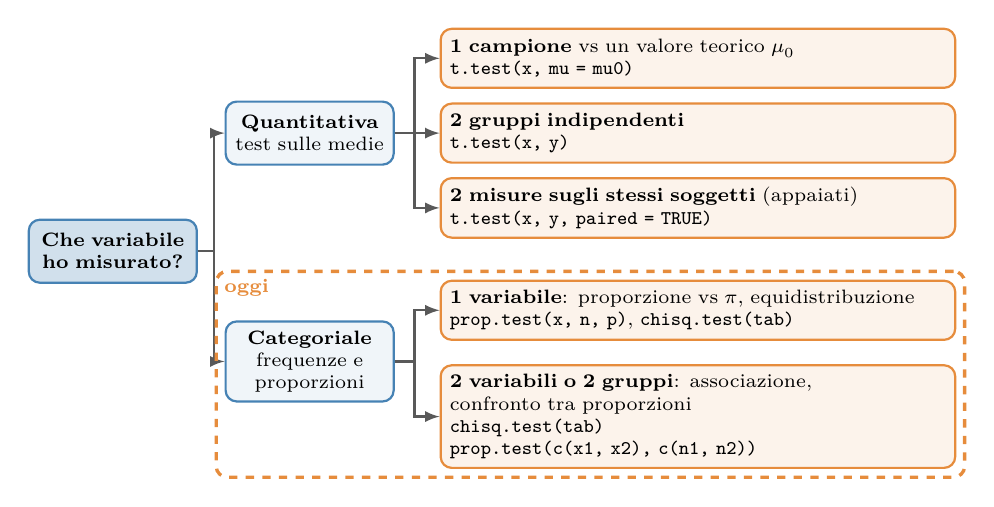
\begin{tikzpicture}[
  dom/.style  = {rectangle, rounded corners, draw = evid, thick, fill = evid!8,
                 align = center, font = \scriptsize, text width = 1.9cm, minimum height = 0.8cm},
  foglia/.style = {rectangle, rounded corners, draw = evidB, thick, fill = evidB!10,
                 align = left, font = \scriptsize, text width = 6.3cm, minimum height = 0.75cm,
                 anchor = west},
  freccia/.style = {-latex, thick, gray!70!black}
]
% radice
\node[dom, fill = evid!25] (rad) at (0,0.1) {\textbf{Che variabile\\ ho misurato?}};

% primo livello
\node[dom] (quant) at (2.5, 1.6)  {\textbf{Quantitativa}\\ test sulle medie};
\node[dom] (cat)   at (2.5, -1.3) {\textbf{Categoriale}\\ frequenze e\\ proporzioni};
\draw[freccia] (rad.east) -- ++(0.2,0) |- (quant.west);
\draw[freccia] (rad.east) -- ++(0.2,0) |- (cat.west);

% foglie: variabile quantitativa
\node[foglia] (t1) at (4.15, 2.55) {\textbf{1 campione} vs un valore teorico $\mu_0$\\ \texttt{t.test(x, mu = mu0)}};
\node[foglia] (t2) at (4.15, 1.6)  {\textbf{2 gruppi indipendenti}\\ \texttt{t.test(x, y)}};
\node[foglia] (t3) at (4.15, 0.65) {\textbf{2 misure sugli stessi soggetti} (appaiati)\\ \texttt{t.test(x, y, paired = TRUE)}};
\foreach \f in {t1, t2, t3}
  \draw[freccia] (quant.east) -- ++(0.25,0) |- (\f.west);

% foglie: variabile categoriale
\node[foglia] (c1) at (4.15, -0.65) {\textbf{1 variabile}: proporzione vs $\pi$, equidistribuzione\\ \texttt{prop.test(x, n, p)}, \texttt{chisq.test(tab)}};
\node[foglia] (c2) at (4.15, -2.0) {\textbf{2 variabili o 2 gruppi}: associazione,\\ confronto tra proporzioni\\ \texttt{chisq.test(tab)}\\ \texttt{prop.test(c(x1, x2), c(n1, n2))}};
\foreach \f in {c1, c2}
  \draw[freccia] (cat.east) -- ++(0.25,0) |- (\f.west);

% la parte di oggi
\uncover<2->{
\node[draw = evidB, very thick, dashed, rounded corners, inner sep = 3pt, fit = (cat)(c1)(c2)] (box) {};
\node[font = \scriptsize\bfseries, text = evidB, anchor = north west] at (box.north west) {oggi};
}
\end{tikzpicture}
\end{frame}

\section{Test Chi-quadrato}\label{test-chi-quadrato}

\subsection{Associazione tra due
variabili}\label{associazione-tra-due-variabili}

\begin{frame}{}
\phantomsection\label{section}
\begin{tcolorbox}[enhanced jigsaw, opacitybacktitle=0.6, colframe=quarto-callout-tip-color-frame, arc=.35mm, colbacktitle=quarto-callout-tip-color!10!white, titlerule=0mm, breakable, colback=white, opacityback=0, coltitle=black, leftrule=.75mm, bottomtitle=1mm, toptitle=1mm, title={Scopo}, bottomrule=.15mm, rightrule=.15mm, toprule=.15mm, left=2mm]

Quantificare il grado di associazione tra due variabili nominali A con
\(I\) categorie e B con \(J\) categorie

\end{tcolorbox}

\[\chi^2 =  \sum_{i} \sum_{j} \displaystyle \frac{(n_{ij} - n_{ij}^*)^2}{n_{ij}^*}\]

\begin{columns}[T]
\begin{column}{0.5\linewidth}
\[n_{ij}^* = \dfrac{n_{i.} \times n_{.j}}{n}\]
\end{column}

\begin{column}{0.5\linewidth}
\[N = \sum_{i=1}^I \sum_{j=1}^J n_{ij}\]
\end{column}
\end{columns}
\end{frame}

\begin{frame}{}
\phantomsection\label{section-1}
Le ipotesi riguardano la popolazione, quindi si formulano sulle
proporzioni nella popolazione:

\begin{itemize}
\tightlist
\item
  \(\pi_{ij}\): proporzione di casi che hanno sia la categoria \(i\) di
  A sia la categoria \(j\) di B
\item
  \(\pi_{i\cdot}\): proporzione di casi nella categoria \(i\) di A
\item
  \(\pi_{\cdot j}\): proporzione di casi nella categoria \(j\) di B
\end{itemize}

Se A e B sono indipendenti, la proporzione congiunta è il prodotto delle
proporzioni marginali: \(\pi_{ij} = \pi_{i\cdot}\,\pi_{\cdot j}\)

È la stessa logica delle frequenze attese calcolate sul campione:

\[\dfrac{n_{ij}^*}{N} = \dfrac{n_{i.}}{n} \times \dfrac{n_{.j}}{n}\]
\end{frame}

\begin{frame}{}
\phantomsection\label{section-2}
\begin{tcolorbox}[enhanced jigsaw, opacitybacktitle=0.6, colframe=quarto-callout-note-color-frame, arc=.35mm, colbacktitle=quarto-callout-note-color!10!white, titlerule=0mm, breakable, colback=white, opacityback=0, coltitle=black, leftrule=.75mm, bottomtitle=1mm, toptitle=1mm, title={Sistema di ipotesi}, bottomrule=.15mm, rightrule=.15mm, toprule=.15mm, left=2mm]

\(H_0\): A e B sono indipendenti nella popolazione, cioè
\(\pi_{ij} = \pi_{i\cdot}\,\pi_{\cdot j}\) per ogni \(i, j\)

\(H_1\): A e B sono associate nella popolazione, cioè
\(\pi_{ij} \neq \pi_{i\cdot}\,\pi_{\cdot j}\) per almeno una coppia
\(i, j\)

\end{tcolorbox}

Se \(H_0\) è vera, ci aspettiamo che le frequenze osservate si
discostino da quelle attese solo per effetto della variabilità
campionaria. Il \(\chi^2\) misura questo scostamento: più è grande, meno
i dati sono compatibili con \(H_0\).
\end{frame}

\subsection{In R}\label{in-r}

\begin{frame}[fragile]{}
\phantomsection\label{section-3}
\begin{longtable}[]{@{}
  >{\raggedright\arraybackslash}p{(\linewidth - 2\tabcolsep) * \real{0.2573}}
  >{\raggedright\arraybackslash}p{(\linewidth - 2\tabcolsep) * \real{0.7427}}@{}}
\toprule\noalign{}
\begin{minipage}[b]{\linewidth}\raggedright
\textbf{Simbolo R}
\end{minipage} & \begin{minipage}[b]{\linewidth}\raggedright
\textbf{Significato}
\end{minipage} \\
\midrule\noalign{}
\endhead
\texttt{chisq.test(mytab)} & Calcola il test statistico del chi quadro
alla tabella di frequenze chiamata \texttt{mytab} \\
\bottomrule\noalign{}
\end{longtable}

\begin{Shaded}
\begin{Highlighting}[]
\NormalTok{mytable }\OtherTok{\textless{}{-}} \FunctionTok{matrix}\NormalTok{(}\FunctionTok{c}\NormalTok{(}\DecValTok{21}\NormalTok{,}\DecValTok{9}\NormalTok{,}\DecValTok{9}\NormalTok{,}\DecValTok{33}\NormalTok{,}\DecValTok{10}\NormalTok{,}\DecValTok{28}\NormalTok{,}\DecValTok{7}\NormalTok{,}\DecValTok{12}\NormalTok{,}\DecValTok{10}\NormalTok{),}\DecValTok{3}\NormalTok{,}\DecValTok{3}\NormalTok{)}
\FunctionTok{rownames}\NormalTok{(mytable) }\OtherTok{\textless{}{-}} \FunctionTok{c}\NormalTok{(}\StringTok{"a1"}\NormalTok{,}\StringTok{"a2"}\NormalTok{,}\StringTok{"a3"}\NormalTok{)}
\FunctionTok{colnames}\NormalTok{(mytable) }\OtherTok{\textless{}{-}} \FunctionTok{c}\NormalTok{(}\StringTok{"b1"}\NormalTok{,}\StringTok{"b2"}\NormalTok{,}\StringTok{"b3"}\NormalTok{)}
\FunctionTok{chisq.test}\NormalTok{(mytable)}
\end{Highlighting}
\end{Shaded}
\end{frame}

\subsection{Esempi}\label{esempi}

\begin{frame}[fragile]{}
\phantomsection\label{section-4}
\begin{Shaded}
\begin{Highlighting}[]
\FunctionTok{chisq.test}\NormalTok{(mytable)}
\end{Highlighting}
\end{Shaded}

\begin{verbatim}

    Pearson's Chi-squared test

data:  mytable
X-squared = 12.458, df = 4, p-value = 0.01425
\end{verbatim}
\end{frame}

\begin{frame}[fragile]{}
\phantomsection\label{section-5}
\begin{Verbatim}[commandchars=\\\{\}, fontsize=\scriptsize, frame=single, framesep=2mm]
> chisq.test(mytable)
\tikzmarknode{test}{Pearson's Chi-squared test}

data:  mytable
\tikzmarknode{stat}{X-squared = 12.458}, \tikzmarknode{df}{df = 4}, \tikzmarknode{pval}{p-value = 0.01425}
\end{Verbatim}

\begin{tikzpicture}[remember picture, overlay,
  box/.style={draw=unipd, very thick, rounded corners=3pt, inner sep=1.5pt},
  num/.style={circle, fill=unipd, text=white, font=\tiny\bfseries,
              inner sep=0pt, minimum size=9pt}]
  {\node[box, fit=(test)] (b1) {}; \node[num] at (b1.north east) {1};}
  {\node[box, fit=(stat)] (b2) {}; \node[num] at (b2.north east) {2};}
  {\node[box, fit=(df)] (b3) {}; \node[num] at (b3.north east) {3};}
  {\node[box, fit=(pval)] (b4) {}; \node[num] at (b4.north east) {4};}
\end{tikzpicture}
\vspace{-3mm}
\begin{columns}[T]
\begin{column}{.48\textwidth}
\footnotesize
\begin{enumerate}
  \item Tipo di test
  \item Statistica test $\chi^2_0$
\end{enumerate}
\end{column}
\begin{column}{.48\textwidth}
\footnotesize
\begin{enumerate}
  \setcounter{enumi}{2}
  \item Gradi di libertà: $df = (I - 1)(J - 1)$
  \item $p$-value: area a destra di $\chi^2_0$
\end{enumerate}
\end{column}
\end{columns}
\end{frame}

\begin{frame}[fragile]{}
\phantomsection\label{section-6}
\small

\[p\text{-value} = 1- \int_{-\infty}^{\chi_0} f_x(x|\theta)dx\]

\begin{center}
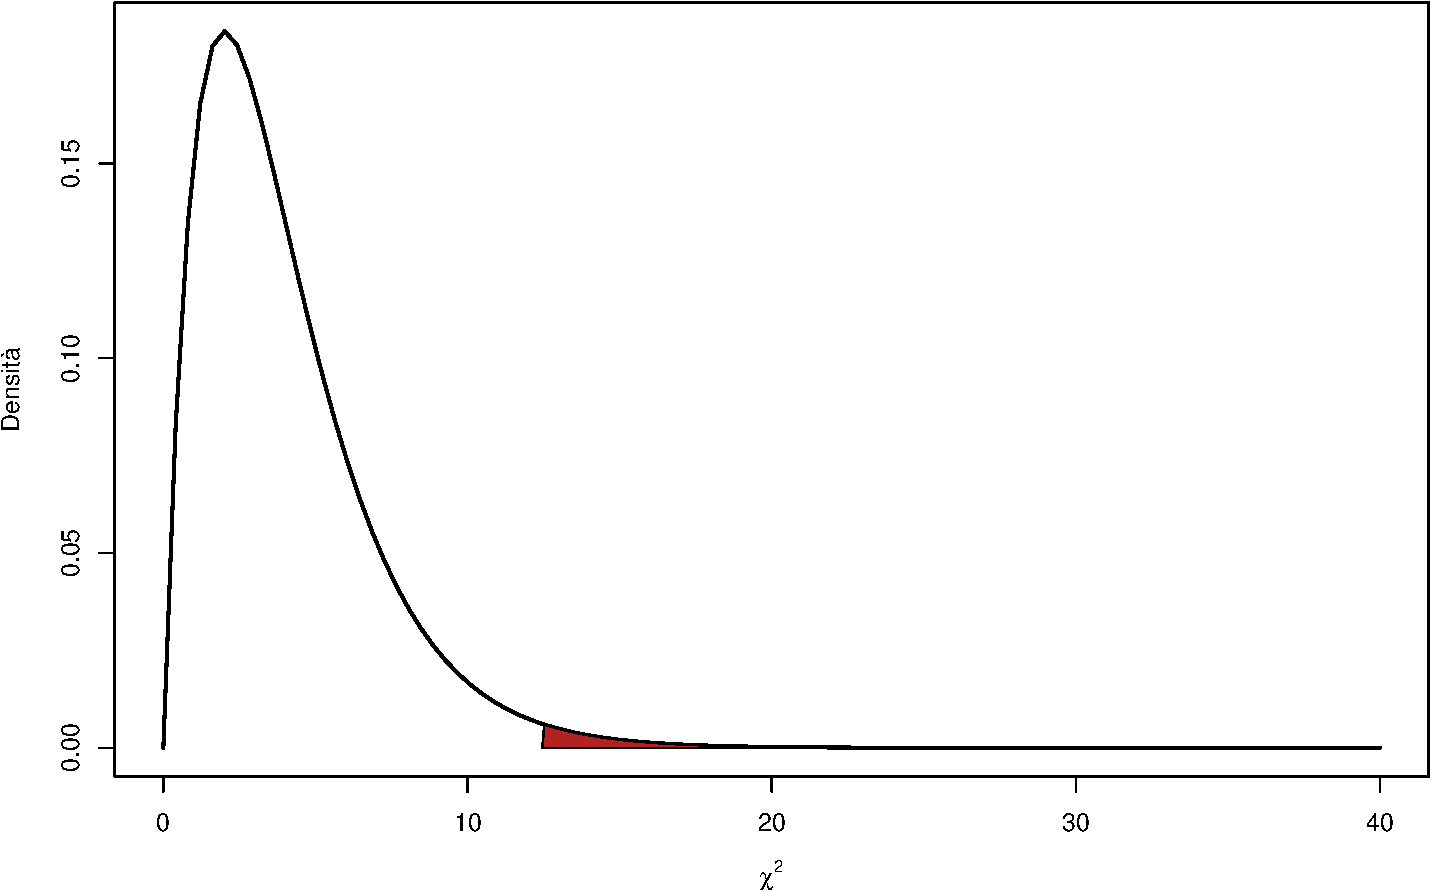
\includegraphics[width=0.6\linewidth,height=\textheight,keepaspectratio]{modulo6-b-bozza-commenti_files/figure-beamer/unnamed-chunk-5-1.pdf}
\end{center}

\begin{Shaded}
\begin{Highlighting}[]
\DecValTok{1}\SpecialCharTok{{-}}\FunctionTok{pchisq}\NormalTok{(}\FloatTok{12.458}\NormalTok{, }\DecValTok{4}\NormalTok{)}
\end{Highlighting}
\end{Shaded}

\begin{verbatim}
[1] 0.01425141
\end{verbatim}
\end{frame}

\subsection{Equidistribuzione nelle
categorie}\label{equidistribuzione-nelle-categorie}

\begin{frame}{}
\phantomsection\label{section-7}
\begin{tcolorbox}[enhanced jigsaw, opacitybacktitle=0.6, colframe=quarto-callout-tip-color-frame, arc=.35mm, colbacktitle=quarto-callout-tip-color!10!white, titlerule=0mm, breakable, colback=white, opacityback=0, coltitle=black, leftrule=.75mm, bottomtitle=1mm, toptitle=1mm, title={Scopo}, bottomrule=.15mm, rightrule=.15mm, toprule=.15mm, left=2mm]

Valutare se le proporzioni nelle \(I\) categorie di una variabile
categoriale \(A\) siano o meno conformi a un modello teorico
(solitamente di omogeneità)

\end{tcolorbox}

\[\chi^2 =  \sum_{i} \displaystyle \frac{(n_{i} - n_{i}^*)^2}{n_{i}^*}\]

\begin{columns}[T]
\begin{column}{0.5\linewidth}
Frequenze attese sotto il modello teorico di omogeneità

\[n_{i}^* = \dfrac{1}{I}n\]
\end{column}

\begin{column}{0.5\linewidth}
Frequenze osservate per le \(I\) categorie

\[n = \sum_{i=1}^I n_{i}\]
\end{column}
\end{columns}
\end{frame}

\begin{frame}{}
\phantomsection\label{section-8}
Indichiamo con \(\pi_i\) la proporzione di casi nella categoria \(i\) di
A nella popolazione.

\begin{tcolorbox}[enhanced jigsaw, opacitybacktitle=0.6, colframe=quarto-callout-note-color-frame, arc=.35mm, colbacktitle=quarto-callout-note-color!10!white, titlerule=0mm, breakable, colback=white, opacityback=0, coltitle=black, leftrule=.75mm, bottomtitle=1mm, toptitle=1mm, title={Sistema di ipotesi}, bottomrule=.15mm, rightrule=.15mm, toprule=.15mm, left=2mm]

\(H_0\): le proporzioni nelle \(I\) categorie sono uguali nella
popolazione, cioè \(\pi_i = 1/I\) per ogni \(i\)

\(H_1\): nella popolazione almeno una proporzione è diversa da \(1/I\),
cioè \(\pi_i \neq 1/I\) per almeno un \(i\)

\end{tcolorbox}

Se \(H_0\) è vera, ci aspettiamo che le frequenze osservate si
discostino da quelle attese solo per effetto della variabilità
campionaria. Il \(\chi^2\) misura questo scostamento: più è grande, meno
i dati sono compatibili con \(H_0\).
\end{frame}

\subsection{In R}\label{in-r-1}

\begin{frame}[fragile,plain]{}
\phantomsection\label{section-9}
\small

\begin{longtable}[]{@{}
  >{\raggedright\arraybackslash}p{(\linewidth - 2\tabcolsep) * \real{0.2573}}
  >{\raggedright\arraybackslash}p{(\linewidth - 2\tabcolsep) * \real{0.7427}}@{}}
\toprule\noalign{}
\begin{minipage}[b]{\linewidth}\raggedright
\textbf{Simbolo R}
\end{minipage} & \begin{minipage}[b]{\linewidth}\raggedright
\textbf{Significato}
\end{minipage} \\
\midrule\noalign{}
\endhead
\texttt{chisq.test(mytab)} & Calcola il test statistico del chi quadro
alla tabella di frequenze chiamata \texttt{mytab} \\
\bottomrule\noalign{}
\end{longtable}

\footnotezize

\begin{Shaded}
\begin{Highlighting}[]
\NormalTok{mytable }\OtherTok{\textless{}{-}} \FunctionTok{matrix}\NormalTok{(}\FunctionTok{c}\NormalTok{(}\DecValTok{22}\NormalTok{,}\DecValTok{45}\NormalTok{,}\DecValTok{18}\NormalTok{),}\DecValTok{1}\NormalTok{,}\DecValTok{3}\NormalTok{)}
\FunctionTok{colnames}\NormalTok{(mytable) }\OtherTok{\textless{}{-}} \FunctionTok{c}\NormalTok{(}\StringTok{"a1"}\NormalTok{,}\StringTok{"a2"}\NormalTok{,}\StringTok{"a3"}\NormalTok{)}
\FunctionTok{chisq.test}\NormalTok{(mytable)}
\end{Highlighting}
\end{Shaded}

\begin{verbatim}

    Chi-squared test for given probabilities

data:  mytable
X-squared = 14.988, df = 2, p-value = 0.0005563
\end{verbatim}
\end{frame}

\subsection{Esempi}\label{esempi-1}

\begin{frame}[fragile]{}
\phantomsection\label{section-10}
\begin{Shaded}
\begin{Highlighting}[]
\FunctionTok{chisq.test}\NormalTok{(mytable)}
\end{Highlighting}
\end{Shaded}

\begin{verbatim}

    Chi-squared test for given probabilities

data:  mytable
X-squared = 14.988, df = 2, p-value = 0.0005563
\end{verbatim}
\end{frame}

\begin{frame}[fragile]{}
\phantomsection\label{section-11}
\begin{Verbatim}[commandchars=\\\{\}, fontsize=\scriptsize, frame=single, framesep=2mm]
> chisq.test(mytable)
\tikzmarknode{test}{Chi-squared test for given probabilities}

data:  mytable
\tikzmarknode{stat}{X-squared = 14.988}, \tikzmarknode{df}{df = 2}, \tikzmarknode{pval}{p-value = 0.0005563}
\end{Verbatim}

\begin{tikzpicture}[remember picture, overlay,
  box/.style={draw=unipd, very thick, rounded corners=3pt, inner sep=1.5pt},
  num/.style={circle, fill=unipd, text=white, font=\tiny\bfseries,
              inner sep=0pt, minimum size=9pt}]
  {\node[box, fit=(test)] (b1) {}; \node[num] at (b1.north east) {1};}
  {\node[box, fit=(stat)] (b2) {}; \node[num] at (b2.north east) {2};}
  {\node[box, fit=(df)] (b3) {}; \node[num] at (b3.north east) {3};}
  {\node[box, fit=(pval)] (b4) {}; \node[num] at (b4.north east) {4};}
\end{tikzpicture}
\vspace{-3mm}
\begin{columns}[T]
\begin{column}{.48\textwidth}
\footnotesize
\begin{enumerate}
  \item Tipo di test
  \item Statistica test $\chi^2_0$
\end{enumerate}
\end{column}
\begin{column}{.48\textwidth}
\footnotesize
\begin{enumerate}
  \setcounter{enumi}{2}
  \item Gradi di libertà: $df = I - 1$
  \item $p$-value: area a destra di $\chi^2_0$
\end{enumerate}
\end{column}
\end{columns}
\end{frame}

\section{Altri test per variabili
categoriali}\label{altri-test-per-variabili-categoriali}

\subsection{Test delle proporzioni}\label{test-delle-proporzioni}

\begin{frame}[fragile]{Una proporzione}
\phantomsection\label{una-proporzione}
\begin{tcolorbox}[enhanced jigsaw, opacitybacktitle=0.6, colframe=quarto-callout-tip-color-frame, arc=.35mm, colbacktitle=quarto-callout-tip-color!10!white, titlerule=0mm, breakable, colback=white, opacityback=0, coltitle=black, leftrule=.75mm, bottomtitle=1mm, toptitle=1mm, title={Scopo}, bottomrule=.15mm, rightrule=.15mm, toprule=.15mm, left=2mm]

Valutare se la proporzione \(\pi\) di successi nella popolazione sia
diversa (rispettivamente maggiore o minore) da un valore teorico
\(\pi_0\)

\end{tcolorbox}

\textbf{Stimatore} di \(\pi\): \(x/n\), proporzione di successi su \(n\)
prove indipendenti. In \texttt{prop.test()}, \(\pi_0\) è l'argomento
\texttt{p}

\begin{tcolorbox}[enhanced jigsaw, opacitybacktitle=0.6, colframe=quarto-callout-note-color-frame, arc=.35mm, colbacktitle=quarto-callout-note-color!10!white, titlerule=0mm, breakable, colback=white, opacityback=0, coltitle=black, leftrule=.75mm, bottomtitle=1mm, toptitle=1mm, title={Sistema di ipotesi}, bottomrule=.15mm, rightrule=.15mm, toprule=.15mm, left=2mm]

Due code: \(H_0: \pi = \pi_0 \qquad H_1: \pi \neq \pi_0\)

Una coda destra: \(H_0: \pi = \pi_0 \qquad H_1: \pi > \pi_0\)

Una coda sinistra: \(H_0: \pi = \pi_0 \qquad H_1: \pi < \pi_0\)

\end{tcolorbox}
\end{frame}

\begin{frame}{Due proporzioni}
\phantomsection\label{due-proporzioni}
\begin{tcolorbox}[enhanced jigsaw, opacitybacktitle=0.6, colframe=quarto-callout-tip-color-frame, arc=.35mm, colbacktitle=quarto-callout-tip-color!10!white, titlerule=0mm, breakable, colback=white, opacityback=0, coltitle=black, leftrule=.75mm, bottomtitle=1mm, toptitle=1mm, title={Scopo}, bottomrule=.15mm, rightrule=.15mm, toprule=.15mm, left=2mm]

Valutare se la proporzione di successi \(\pi_1\) di una popolazione sia
diversa (rispettivamente maggiore o minore) dalla proporzione di
successi \(\pi_2\) di un'altra popolazione

\end{tcolorbox}

\textbf{Stimatore} di \(\pi_1 - \pi_2\): \(x_1/n_1 - x_2/n_2\),
differenza tra le proporzioni di successi nei due campioni

\begin{tcolorbox}[enhanced jigsaw, opacitybacktitle=0.6, colframe=quarto-callout-note-color-frame, arc=.35mm, colbacktitle=quarto-callout-note-color!10!white, titlerule=0mm, breakable, colback=white, opacityback=0, coltitle=black, leftrule=.75mm, bottomtitle=1mm, toptitle=1mm, title={Sistema di ipotesi}, bottomrule=.15mm, rightrule=.15mm, toprule=.15mm, left=2mm]

Due code: \(H_0: \pi_1 = \pi_2 \qquad H_1: \pi_1 \neq \pi_2\)

Una coda destra: \(H_0: \pi_1 = \pi_2 \qquad H_1: \pi_1 > \pi_2\)

Una coda sinistra: \(H_0: \pi_1 = \pi_2 \qquad H_1: \pi_1 < \pi_2\)

\end{tcolorbox}
\end{frame}

\begin{frame}[fragile,plain]{}
\phantomsection\label{section-12}
\small

\begin{longtable}[]{@{}
  >{\raggedright\arraybackslash}p{(\linewidth - 2\tabcolsep) * \real{0.3810}}
  >{\raggedright\arraybackslash}p{(\linewidth - 2\tabcolsep) * \real{0.6190}}@{}}
\toprule\noalign{}
\begin{minipage}[b]{\linewidth}\raggedright
\textbf{Funzione R}
\end{minipage} & \begin{minipage}[b]{\linewidth}\raggedright
\textbf{Significato}
\end{minipage} \\
\midrule\noalign{}
\endhead
\texttt{prop.test(x,\ n,\ p)} & Calcola se la proporzione \(x/n\) (dove
\(x \le n\)) sia significativamente differente dal valore di probabilità
\(p\). Il valore \(x\) è il numero di esiti dicotomici positivi su \(n\)
distinte prove (\(\pi \neq \pi_0\)) \\
\texttt{prop.test(x,\ n,\ p,\ alternative\ =\ "less")} & \emph{Test
inferenziale a una coda sinistra} \(\pi < \pi_0\) \\
\texttt{prop.test(x,\ n,\ p,\ alternative\ =\ "greater")} & \emph{Test
inferenziale a una coda destra} \(\pi > \pi_0\) \\
\texttt{prop.test(c(x1,x2),\ c(n1,n2))} & \emph{Test inferenziale a due
code per due proporzioni} \(\pi_1 \neq \pi_2\) \\
\texttt{prop.test(c(x1,x2),\ c(n1,n2),\ alternative\ =\ "less")} &
\emph{Test inferenziale a una coda (sinistra) per due proporzioni}
\(\pi_1 < \pi_2\) \\
\texttt{prop.test(c(x1,x2),\ c(n1,n2),\ alternative\ =\ "greater")} &
\emph{Test inferenziale a una coda (destra) per due proporzioni}
\(\pi_1 > \pi_2\) \\
\bottomrule\noalign{}
\end{longtable}
\end{frame}

\subsection{Esempi: 1 Campione}\label{esempi-1-campione}

\begin{frame}[fragile]{}
\phantomsection\label{section-13}
\small

Campione di bambini che supera (1) o non supera (0) un punteggio minimo
alle matrici di Raven. Nella popolazione a cui appartengono, la
maggioranza degli individui supera la soglia minima alle matrici di
Raven?

\(H_0: \pi = .50 \qquad H_1: \pi > .50\)

\footnotesize

\begin{Shaded}
\begin{Highlighting}[]
\CommentTok{\# Test delle proporzioni}
\NormalTok{pass\_scores }\OtherTok{=} \FunctionTok{c}\NormalTok{(}\DecValTok{1}\NormalTok{,}\DecValTok{0}\NormalTok{,}\DecValTok{0}\NormalTok{,}\DecValTok{1}\NormalTok{,}\DecValTok{1}\NormalTok{,}\DecValTok{0}\NormalTok{,}\DecValTok{0}\NormalTok{,}\DecValTok{0}\NormalTok{,}\DecValTok{0}\NormalTok{,}\DecValTok{1}\NormalTok{,}\DecValTok{0}\NormalTok{,}\DecValTok{1}\NormalTok{,}\DecValTok{0}\NormalTok{,}\DecValTok{1}\NormalTok{,}\DecValTok{0}\NormalTok{,}\DecValTok{0}\NormalTok{) }\CommentTok{\# }
\FunctionTok{table}\NormalTok{(pass\_scores) }\CommentTok{\# Frequenze insuccessi/successi}
\NormalTok{x }\OtherTok{=} \FunctionTok{sum}\NormalTok{(pass\_scores) }\CommentTok{\# x, numero dei successi}
\NormalTok{n }\OtherTok{=} \FunctionTok{length}\NormalTok{(pass\_scores) }\CommentTok{\# n, numero totale di prove indipendenti}
\FunctionTok{prop.test}\NormalTok{(x, }\AttributeTok{n =}\NormalTok{ n, }\AttributeTok{p =}\NormalTok{ .}\DecValTok{50}\NormalTok{, }\AttributeTok{alternative =} \StringTok{"greater"}\NormalTok{) }\CommentTok{\# Test}
\end{Highlighting}
\end{Shaded}
\end{frame}

\begin{frame}[fragile]{}
\phantomsection\label{section-14}
\begin{Verbatim}[commandchars=\\\{\}, fontsize=\scriptsize, frame=single, framesep=2mm]
> prop.test(x, n = n, p = .50, alternative = "greater")
\tikzmarknode{test}{1-sample proportions test with continuity correction}

data:  x out of n, null probability 0.5
\tikzmarknode{stat}{X-squared = 0.5625}, \tikzmarknode{df}{df = 1}, \tikzmarknode{pval}{p-value = 0.7734}
\tikzmarknode{h1}{alternative hypothesis: true p is greater than 0.5}
95 percent confidence interval:
 \tikzmarknode{ic}{0.1843081 1.0000000}
sample estimates:
    p
 \tikzmarknode{stime}{0.375}
\end{Verbatim}

\begin{tikzpicture}[remember picture, overlay,
  box/.style={draw=unipd, very thick, rounded corners=3pt, inner sep=1.5pt},
  num/.style={circle, fill=unipd, text=white, font=\tiny\bfseries,
              inner sep=0pt, minimum size=9pt}]
  {\node[box, fit=(test)] (b1) {}; \node[num] at (b1.north east) {1};}
  {\node[box, fit=(stat)] (b2) {}; \node[num] at (b2.north east) {2};}
  {\node[box, fit=(df)] (b3) {}; \node[num] at (b3.north east) {3};}
  {\node[box, fit=(pval)] (b4) {}; \node[num] at (b4.north east) {4};}
  {\node[box, fit=(h1)] (b5) {}; \node[num] at (b5.north east) {5};}
  {\node[box, fit=(ic)] (b6) {}; \node[num] at (b6.north east) {6};}
  {\node[box, fit=(stime)] (b7) {}; \node[num] at (b7.north east) {7};}
\end{tikzpicture}
\vspace{-3mm}
\begin{columns}[T]
\begin{column}{.48\textwidth}
\footnotesize
\begin{enumerate}
  \item Tipo di test
  \item Statistica test $\chi^2_0$
  \item Gradi di libertà: $df = 1$
  \item $p$-value a una coda
\end{enumerate}
\end{column}
\begin{column}{.48\textwidth}
\footnotesize
\begin{enumerate}
  \setcounter{enumi}{4}
  \item Ipotesi alternativa $H_1$: $\pi > \pi_0$
  \item IC \textbf{unidirezionale} al 95\% per $\pi$
  \item Stimatore di $\pi$: proporzione campionaria $x/n$
\end{enumerate}
\end{column}
\end{columns}
\end{frame}

\subsection{Esempi: 2 campioni}\label{esempi-2-campioni}

\begin{frame}[fragile]{}
\phantomsection\label{section-15}
\begin{columns}[T]
\begin{column}{0.5\linewidth}
\(x_1 = 6\), \(n_1 = 16\)
\end{column}

\begin{column}{0.5\linewidth}
\(x_2 = 21\), \(n_2 = 30\)
\end{column}
\end{columns}

Le proporzioni di successi nei due gruppi sono diverse?

\(H_0: \pi_1 = \pi_2 \qquad H_1: \pi_1 \neq \pi_2\)

\begin{Shaded}
\begin{Highlighting}[]
\NormalTok{x\_2 }\OtherTok{=} \DecValTok{21}
\NormalTok{n\_2 }\OtherTok{=} \DecValTok{30}
\FunctionTok{prop.test}\NormalTok{(}\FunctionTok{c}\NormalTok{(x,x\_2), }\FunctionTok{c}\NormalTok{(n, n\_2), }\AttributeTok{alternative =} \StringTok{"two.sided"}\NormalTok{)}
\end{Highlighting}
\end{Shaded}
\end{frame}

\begin{frame}[fragile]{}
\phantomsection\label{section-16}
\begin{Verbatim}[commandchars=\\\{\}, fontsize=\scriptsize, frame=single, framesep=2mm]
> prop.test(c(x, x_2), c(n, n_2), alternative = "two.sided")
\tikzmarknode{test}{2-sample test for equality of proportions with continuity correction}

data:  c(x, x_2) out of c(n, n_2)
\tikzmarknode{stat}{X-squared = 3.3045}, \tikzmarknode{df}{df = 1}, \tikzmarknode{pval}{p-value = 0.06909}
\tikzmarknode{h1}{alternative hypothesis: two.sided}
95 percent confidence interval:
 \tikzmarknode{ic}{-0.66129416  0.01129416}
sample estimates:
prop 1 prop 2
 \tikzmarknode{stime}{0.375  0.700}
\end{Verbatim}

\begin{tikzpicture}[remember picture, overlay,
  box/.style={draw=unipd, very thick, rounded corners=3pt, inner sep=1.5pt},
  num/.style={circle, fill=unipd, text=white, font=\tiny\bfseries,
              inner sep=0pt, minimum size=9pt}]
  {\node[box, fit=(test)] (b1) {}; \node[num] at (b1.north east) {1};}
  {\node[box, fit=(stat)] (b2) {}; \node[num] at (b2.north east) {2};}
  {\node[box, fit=(df)] (b3) {}; \node[num] at (b3.north east) {3};}
  {\node[box, fit=(pval)] (b4) {}; \node[num] at (b4.north east) {4};}
  {\node[box, fit=(h1)] (b5) {}; \node[num] at (b5.north east) {5};}
  {\node[box, fit=(ic)] (b6) {}; \node[num] at (b6.north east) {6};}
  {\node[box, fit=(stime)] (b7) {}; \node[num] at (b7.north east) {7};}
\end{tikzpicture}
\vspace{-3mm}
\begin{columns}[T]
\begin{column}{.48\textwidth}
\footnotesize
\begin{enumerate}
  \item Tipo di test
  \item Statistica test $\chi^2_0$
  \item Gradi di libertà: $df = 1$
  \item $p$-value
\end{enumerate}
\end{column}
\begin{column}{.48\textwidth}
\footnotesize
\begin{enumerate}
  \setcounter{enumi}{4}
  \item Ipotesi alternativa $H_1$: $\pi_1 \neq \pi_2$
  \item IC al 95\% per $\pi_1 - \pi_2$
  \item Proporzioni campionarie: stimatore $= x_1/n_1 - x_2/n_2$
\end{enumerate}
\end{column}
\end{columns}
\end{frame}




\end{document}
